\documentclass[a4paper,12pt]{beamer}

\usepackage{préambule}
\usetikzlibrary{calc,arrows.meta}

\newcommand{\mysize}{\scriptsize}
\newcommand{\mysizebis}{\tiny}

\newcommand{\myarrow}{{Latex[length=1mm, width=1mm]}-{Latex[length=1mm, width=1mm]}}

\begin{document}

\begin{frame}
	\frametitle{Exercice}

	Pour chaque segment, \textbf{reproduit le sur ton cahier}, puis écrit une expression pour sa longueur, en simplifiant le plus possible : \vspace{0.5cm}

	\begin{tabular}{cc}
		\begin{tikzpicture}
			\coordinate (P1) at (0,0);
			\coordinate (P2) at (1.5,0);
			\coordinate (P3) at (3,0);
			\coordinate (P4) at (4,0);
			\coordinate (P5) at (5,0);

			\draw[|-|] (P1) -- node{\mysizebis /} (P2);
			\draw[|-|] (P2) -- node{\mysizebis /} (P3);
			\draw[|-|] (P3) -- node{\mysizebis //} (P4);
			\draw[|-|] (P4) -- node{\mysizebis //} (P5);

			\draw[\myarrow] ($(P1) - (0,0.3)$) -- node[below] {$x$} ($(P2) - (0,0.3)$);

			\draw[\myarrow] ($(P3) - (0,0.3)$) -- node[below] {2cm} ($(P4) - (0,0.3)$);

			\node at (2.5,-2.5) {. . . . . .};
		\end{tikzpicture} & \hspace{0.7cm} \begin{tikzpicture}
			\coordinate (P1) at (0,0);
			\coordinate (P2) at (1.5,0);
			\coordinate (P3) at (2.5,0);
			\coordinate (P4) at (3.5,0);
			\coordinate (P5) at (5,0);

			\draw[|-|] (P1) -- node{\mysizebis /} (P2);
			\draw[|-|] (P2) -- node{\mysizebis //} (P3);
			\draw[|-|] (P3) -- node{\mysizebis //} (P4);
			\draw[|-|] (P4) -- node{\mysizebis /} (P5);

			\draw[\myarrow] ($(P1) - (0,0.3)$) -- node[below] {$2×x$} ($(P2) - (0,0.3)$);

			\draw[\myarrow] ($(P3) - (0,0.3)$) -- node[below] {3,5cm} ($(P4) - (0,0.3)$);

			\node at (2.5,-2.5) {. . . . . .};
		\end{tikzpicture}
	\end{tabular}
\end{frame}

\begin{frame}
	\frametitle{Exercice}

	Pour chaque figure, \textbf{la reproduire} puis écrire son périmètre en simplifiant le plus possible :

	\begin{tabular}{cc}
		\begin{tikzpicture}
			\newcommand*{\x}{2};
			\newcommand*{\y}{2.5};

			\draw (0,0)
			-- node{\mysize //} ++(\x,0)
			-- node{\mysize /} ++(0,\y)
			-- node{\mysize //} ++(-\x,0)
			-- node{\mysize /} cycle;

			\draw[\myarrow] (0,-0.3) -- node[below] {\small $x$} ++(\x,0);
			\draw[\myarrow] (-0.3,0) -- node[left] {\small $2{,}5$cm} ++(0,\y);

			\node at (\x / 2,-2) {. . . . . .};
		\end{tikzpicture} & 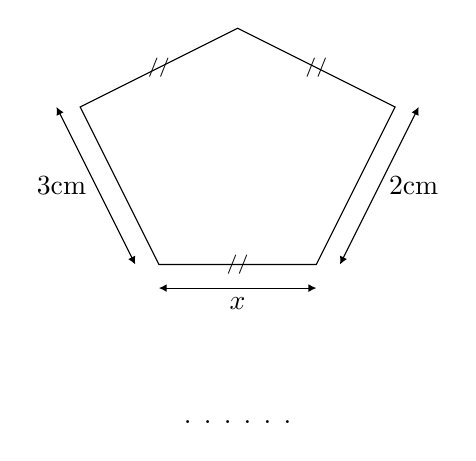
\begin{tikzpicture}
			\coordinate (P1) at (0,0);
			\coordinate (P2) at (2,0);
			\coordinate (P3) at (3,2);
			\coordinate (P4) at (1,3);
			\coordinate (P5) at (-1,2);

			\draw (P1)
			-- node{\mysize //} (P2)
			-- (P3)
			-- node{\mysize //} (P4)
			-- node{\mysize //} (P5)
			-- cycle;

			\draw[\myarrow] ($(P1) - (0,0.3)$) -- node[below] {$x$} ($(P2) - (0,0.3)$);

			\draw[\myarrow] ($(P5) - (0.3,0)$) -- node[left] {3cm} ($(P1) - (0.3,0)$);
			\draw[\myarrow] ($(P2) + (0.3,0)$) -- node[right] {2cm} ($(P3) + (0.3,0)$);

			\node at (1,-2) {. . . . . .};
		\end{tikzpicture}
	\end{tabular}
\end{frame}

\begin{frame}
	\frametitle{Exercice}

	Simplifie les expressions suivantes :

	\begin{itemize}
		\setlength\itemsep{1em}
		\item $0×x + 5 + 2×x =$ \dotfill
		\item $4×x + 3×4 =$ \dotfill
		\item $5×x + 1 + 2×x + 3 =$ \dotfill
		\item $0×x + 1×x + 2×y - 2×y =$ \dotfill
		\item $2{,}5×x - (2 + 1{,}5×x) + 2 =$ \dotfill
	\end{itemize}
\end{frame}

\end{document}